% \documentclass[acmsmall,screen,review,anonymous]{acmart}
\documentclass[sigconf,review,anonymous]{acmart}
\usepackage{amsmath,amsfonts}
\usepackage{algorithmic}
\usepackage{graphicx}
\usepackage{textcomp}
\usepackage{hyperref}
\usepackage{pifont}
\usepackage{caption}
\usepackage{geometry}
\usepackage{longtable}
\usepackage{array}
\usepackage{booktabs}
\usepackage{enumitem}
\usepackage{multirow}
\usepackage{listings}
\usepackage{todonotes}
\usepackage{tcolorbox}
\usepackage{lipsum}
\usepackage{algorithm}
\usepackage{colortbl}
\usepackage{rotating}
\usepackage{booktabs}
\usepackage{multicol}
\usepackage{minted} % Requires --shell-escape flag for compilation
\usepackage{titlesec}
\usepackage{xcolor}
\usepackage[utf8]{inputenc}
\usepackage{lmodern}
\usepackage[T1]{fontenc}

\usepackage{colortbl}
\usepackage{pifont}
\usepackage{graphicx}
\newcommand{\cmark}{\ding{51}} % Check mark
\newcommand{\xmark}{\ding{55}} % X mark
\newcommand{\pmark}{\ding{115}} % Triangle



% Define Colors
\definecolor{bluebox}{HTML}{E3F2FD}   % Light Blue
\definecolor{redbox}{HTML}{FFEBEE}    % Light Red
\definecolor{greenbox}{HTML}{E8F5E9}  % Light Green
\definecolor{graybox}{HTML}{ECEFF1}   % Light Gray
\definecolor{titlecolor}{HTML}{1A237E} % Dark Blue for Headers
\definecolor{codebg}{HTML}{FAFAFA}    % Light Gray for Code

\lstdefinestyle{customc}{
  belowcaptionskip=1\baselineskip,
  breaklines=true,
  frame=L,
  xleftmargin=\parindent,
  language=C,
  showstringspaces=false,
  numbers=left,               % Adds line numbers
  numberstyle=\tiny\color{gray}, % Style for line numbers
  stepnumber=1,
  basicstyle=\tiny\ttfamily, % Reduced font size for the code blocks
  keywordstyle=\bfseries\color{green!40!black},
  commentstyle=\itshape\color{purple!40!black},
  numbersep=8pt,
  identifierstyle=\color{blue},
  stringstyle=\color{orange},
}

\newboolean{showcomments}
\setboolean{showcomments}{true}
\ifthenelse{\boolean{showcomments}}
{\newcommand{\mynote}[2]{
  \fbox{\bfseries\sffamily\scriptsize#1}
  {\small
  $\blacktriangleright$
  \textsf{\textcolor{red}{{#2}}}
  $\blacktriangleleft$}}
}

\newcommand{\az}[1]{\mynote{AZ}{#1}}
\newcommand{\mv}[1]{\mynote{MV}{#1}}

% Define custom colors
\definecolor{lightgreen}{HTML}{98FB98}
\definecolor{lightyellow}{HTML}{FFFF99}
\definecolor{lightred}{HTML}{FFB6C1}

% Define a new environment for numbered paragraphs
\newlist{numpar}{enumerate}{1}
\setlist[numpar,1]{label=\arabic*)}

% Remove the ACM headers and footers
\settopmatter{printacmref=false} % Removes the ACM reference format
\renewcommand\footnotetextcopyrightpermission[1]{} % Removes the copyright notice
\pagestyle{fancy}
% \fancyhf{} % Clear all header and footer fields
% \renewcommand{\headrulewidth}{0pt} % Remove header rule
\acmConference[]{}{}{} % Clears the conference information


% Define custom colors for CODE
\definecolor{bgcolor}{rgb}{0.95,0.95,0.95}  % Light gray background
\definecolor{codeblue}{rgb}{0.0, 0.0, 0.6}  % Keywords in blue
\definecolor{codered}{rgb}{0.6, 0.0, 0.0}   % Strings in red
\definecolor{codegray}{rgb}{0.5, 0.5, 0.5}  % Comments in gray


\begin{document}

\title{Reasoning Challenges for LLMs in Zero-Shot Vulnerability Detection}

\author{Arastoo Zibaeirad}
\affiliation{%
  \institution{University of North Carolina at Charlotte}
  \city{Charlotte}
  \state{NC}
  \country{USA}
}
\email{azibaeir@charlotte.edu}

\author{Marco Vieira}
\affiliation{%
  \institution{University of North Carolina at Charlotte}
  \city{Charlotte}
  \state{NC}
  \country{USA}
}
\email{marco.vieira@charlotte.edu}

\begin{abstract}
Automating software vulnerability detection (SVD) remains a critical challenge in an era of increasingly complex and interdependent software systems. Despite significant advances in Large Language Models (LLMs) for code analysis, prevailing evaluation methodologies often lack the \textbf{context-aware robustness} necessary to capture real-world intricacies and cross-component interactions. To address these limitations, we present \textbf{VulnSage}—a comprehensive evaluation framework and dataset curated from diverse, large-scale open-source system projects. Unlike prior datasets, VulnSage leverages an automated denoising process, incorporating heuristic pre-filtering and NLP-based Git diff classification to ensure a representative yet noise-minimized spectrum of vulnerabilities. Our framework rigorously assesses LLMs using a multi-granular analysis across function, file, and inter-function levels, employing zero-shot prompt strategies: Baseline, Chain-of-Thought, Think, and Think \& Verify. The latter two explicitly test LLMs' reasoning capabilities by requiring structured analysis, evidence-based conclusions, and self-verification.\textcolor{blue}{RESULTS: Through this evaluation, we uncover}
\end{abstract}

\keywords{Vulnerability Detection, Large Language Models, Software Security}



\maketitle

\section{Introduction}
\begin{figure*}[htbp]
    \centering
    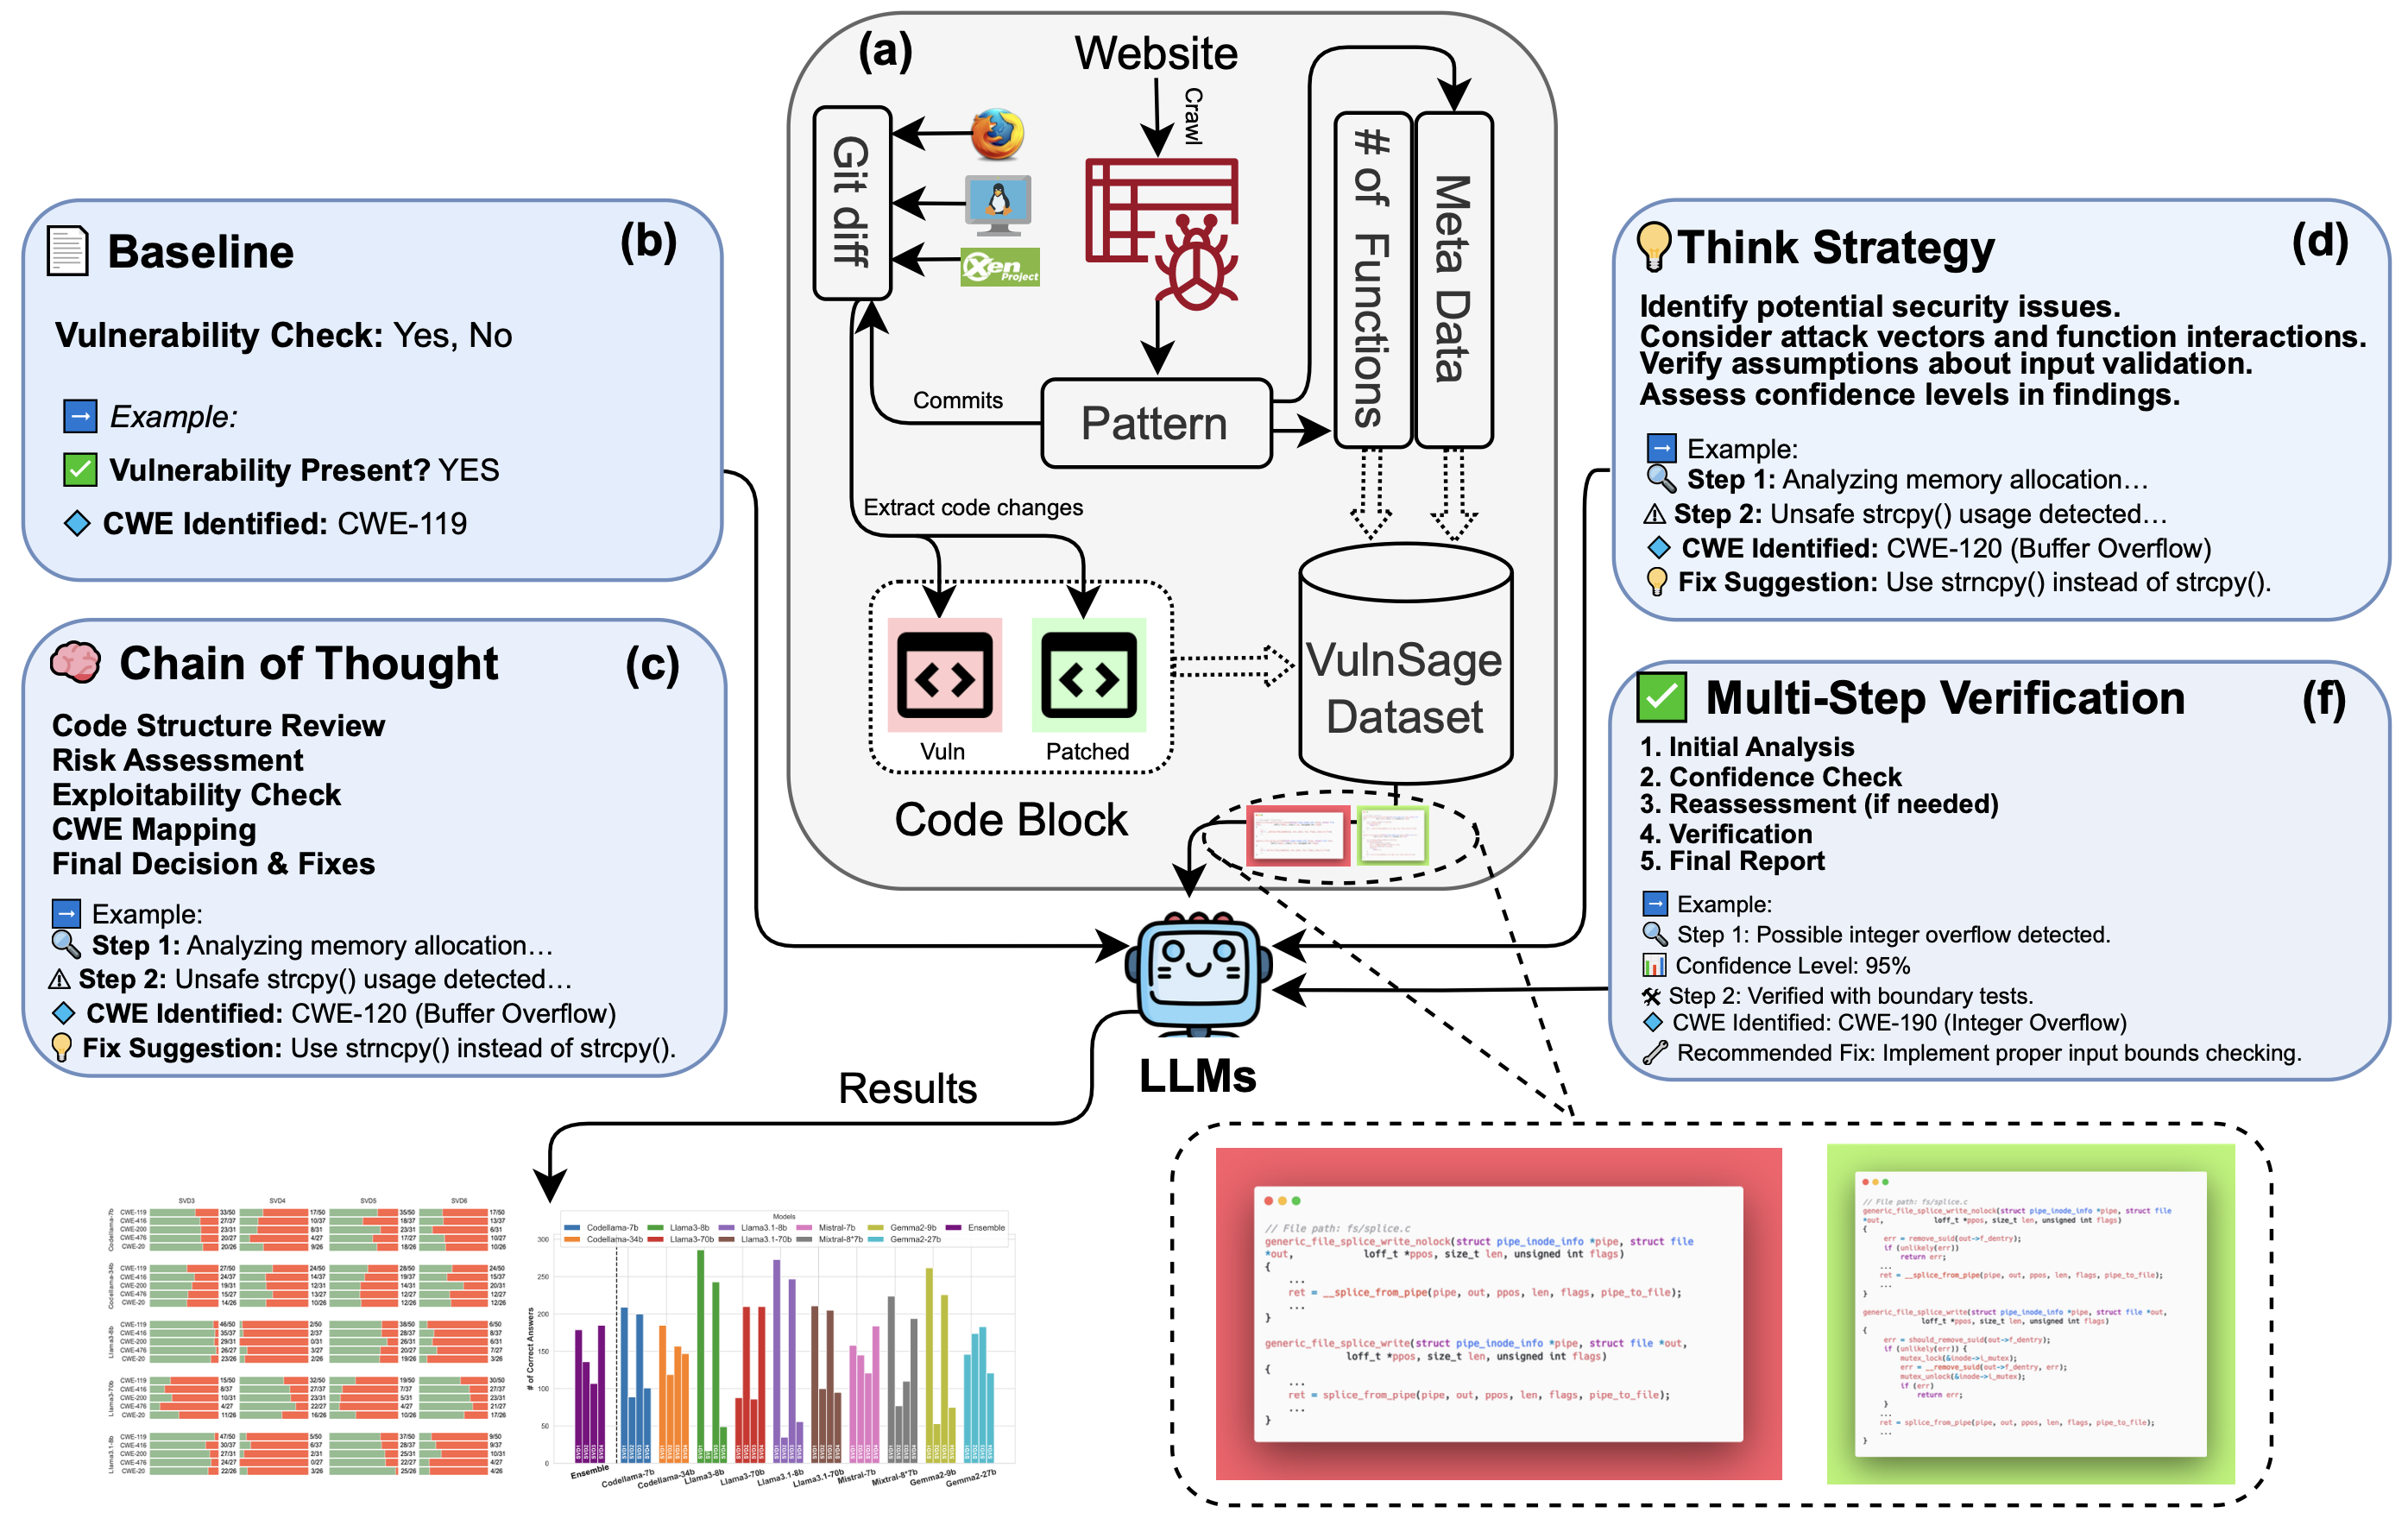
\includegraphics[width=1.0\linewidth]{landing2.png}
    \caption{VulnSage Architecture}
    \label{figure:framework}
\end{figure*}

Automated software vulnerability detection (SVD) is a cornerstone of modern software security, yet traditional program analysis techniques—such as static and dynamic tools—are increasingly challenged by high false positive rates, complex dependency graphs, and limited coverage \cite{manes2019art, klees2018evaluating, pereira2021machine, li2024llm}. These limitations are exacerbated in contemporary software ecosystems, where vulnerabilities often emerge from intricate inter-component interactions and subtle semantic flaws.

Recent breakthroughs in Large Language Models (LLMs) \cite{chen2021evaluating, dubey2024llama, guo2025deepseek} have unlocked strong potentials in code comprehension and semantic reasoning \cite{guo2024deepseek, roziere2023code}. Their ability to analyze code in a context-aware manner offers a promising avenue for SVD. However, critical gaps remain: Can LLMs generalize to real-world vulnerabilities? Are they robust against noisy and incomplete data? Do they reliably detect both common (e.g., CWE-119, CWE-20) and complex vulnerabilities?

To address these questions, we introduce \textbf{VulnSage}, a comprehensive evaluation framework and dataset designed for rigorous benchmarking of LLMs in SVD. VulnSage comprises 594 vulnerabilities across 52 CWE categories, assembled via a rigorous curation process that involves crawling CVEDetails, extracting metadata (commit hashes, CVE, and CWE), and unifying vulnerable code blocks with corresponding patches. To minimize noise, we employ heuristic pre-filtering and NLP-based Git diff classification. Our dataset is publicly available and designed to be extensible for integrating additional projects.

Our evaluation workflow employs a multi-granular approach, analyzing vulnerabilities beyond isolated function- and file-level perspectives to provide a more comprehensive assessment of LLMs' detection capabilities. Instead of treating functions or files as independent units, we construct code blocks that incorporate file paths and inter-function relationships within each file, making the dataset more representative of modern software structures. This approach reflects real-world vulnerability patterns, where security flaws often arise from interactions between multiple functions within a file or across files, rather than existing in isolation. By capturing these dependencies, execution flows, and shared resources, we ensure that LLMs are evaluated on their ability to detect vulnerabilities not only within individual functions or files but also in their contextual interplay.

By deploying twelve LLMs with four sophisticated zero-shot prompt strategies—Baseline, Chain-of-Thought, Think, and Think \& Verify—we rigorously assess the precision of LLMs in distinguishing vulnerable code from fixed versions and systematically examine their potential biases toward specific CWE classes. This comprehensive framework elucidates the models' capabilities in reasoning while exposing their limitations when confronted with complex, cross-component vulnerabilities.

\section{Related Work}
\label{section:related_work}

\subsection{Vulnerability Detection Datasets}
The gold standard for assembling vulnerability datasets has traditionally relied on synthetic benchmarks or crawling repositories such as the National Vulnerability Database (NVD) for fix commits \cite{bhandari2021cvefixes, chakraborty2021deep, pereira2022software, chen2023diversevul}. Researchers typically extract modified files or functions and employ pre-commit analysis to isolate security-related changes. However, this method often introduces significant noise from unrelated modifications (e.g., refactoring, documentation updates) \cite{iannone2022secret, croft2022noisy}. Prior efforts to mitigate noise have relied either on manual annotation—which is labor-intensive and non-scalable—or on simple heuristic filters that do not provide a quantitative assessment of noise \cite{zhou2019devign, hommersom2024automated, gao2023far, siddiq2022securityeval, fan2020ac}.

In contrast, our approach implements a two-tiered noise mitigation strategy. First, we automatically filter out noisy samples by excluding commits with excessive file changes or modifications that are predominantly comments or instructions. Next, we employ a reasoner LLM to evaluate the remaining git diffs and commit descriptions, assigning each a quantitative noise score on a 0–100\% scale. This score serves as an objective metric to assess the residual noise in our dataset. By correlating these noise scores with the performance of LLMs on vulnerability detection tasks, we can systematically evaluate how noise impacts detection capabilities. Moreover, while existing datasets often concentrate on a single granularity—be it at the line level \cite{fu2022linevul}, function level \cite{zhou2019devign, chakraborty2021deep, chen2023diversevul}, file level \cite{liu2024vuldetectbench}, or repository level \cite{zhou2024comparison}—and consequently fail to capture the multifaceted nature of real-world software, our dataset provides a comprehensive and holistic code representation that encapsulates intricate multi-component vulnerability paths.

\subsection{Language Models in Vulnerability Detection}
The advent of LLMs has significantly advanced SVD by enhancing code comprehension and semantic reasoning \cite{ullah2024llms, zibaeirad2024vulnllmeval}. Nonetheless, most current evaluations are conducted on synthetic datasets or via isolated function-level analyses \cite{khare2023understanding}, thereby neglecting  the complexities of cross-component interactions and the impact of noise on detection performance. Additionally, many benchmarks suffer from data leakage issues, as test sets often contain code snippets that appear in LLM training data \cite{sallou2024breaking, wu2023effective}, and they typically focus on common vulnerability patterns, thereby neglecting a diverse range of CWEs \cite{ullah2024llms, wu2023effective}.

Our work addresses these limitations by evaluating LLMs across multiple granularities—function, file, cross-function, and cross-file—to provide a more realistic assessment of their capabilities in detecting subtle, system-level vulnerabilities. Furthermore, by correlating the quantitative noise scores from our two-tiered filtering process with detection performance, we evaluate how noise affects LLM-based vulnerability detection. To mitigate data leakage, we ensure that our test data comprises new samples released after the LLMs' training cutoff dates. Finally, with coverage spanning 52 diverse CWEs, our benchmark offers a rigorous and comprehensive evaluation of LLM effectiveness in real-world security-critical applications. 

\section{Experimental Setup}
\label{section: Experimental Setup}

\subsection{VulnSage Data Collection}
\label{subsection:dataset}
% context limits less than 500 lines >>> convert to ~ 8k tokens
To build VulnSage, we collect vulnerability metadata from the Linux Kernel, Mozilla, and Xen. Using sources like CVEDetails, we gather commit hashes, CVEs, and CWEs. This allows us to track vulnerabilities from discovery to patching, ensuring a structured dataset that supports analysis of how vulnerabilities evolve and are mitigated in real-world software development.

Once metadata is collected, we extract vulnerable and patched code blocks by leveraging commit hashes and file paths to retrieve both the pre-patch (vulnerable) and post-patch (fixed) versions of code from the repository. Each commit is analyzed to build vulnerable and patched code blocks, consisting of files and functions corresponding to a vulnerability, ensuring a structured representation of security flaws. This level of granularity ensures that each vulnerability is captured in its full context rather than as an isolated function or line of code.

To ensure dataset quality, we implement a noise filtration process. After extracting commit hashes and metadata, we automatically remove samples with excessive file and function changes and ignore commits that primarily add or delete comments. To further assess noise, we analyze commit descriptions and patch files (git diff). Commit messages provide contextual insights, while patch files capture the exact modifications. We employ reasoning LLMs to evaluate both sources and assign a noise score, filtering out unrelated changes and ensuring a clean, reliable dataset for vulnerability detection.

In constructing VulnSage, we prioritize diversity and representativeness, encompassing 52 CWEs and 594 unique CVEs. The dataset spans a wide range of vulnerabilities, from minor modifications involving a few lines to extensive patches affecting hundreds of lines of code. This variation in scale and complexity ensures that VulnSage serves as a rigorous and comprehensive benchmark for evaluating LLMs in software vulnerability detection tasks, providing realistic challenges that align with real-world security concerns. 

\subsection{Prompt Templates}
\label{subsection:prompts}
To systematically evaluate LLMs for software vulnerability detection, we employ four distinct prompt strategies, each designed to assess different aspects of reasoning and detection effectiveness. These prompts range from simple binary classification to structured reasoning and verification mechanisms, allowing for a nuanced analysis of LLMs' strengths and limitations in vulnerability detection.

The \textbf{Baseline Prompt} (P1) is a straightforward, direct approach that asks the model whether a specific CWE exists in the given code without requiring explanations or reasoning. This serves as a control to evaluate how well LLMs can detect vulnerabilities without additional reasoning scaffolding.

The \textbf{Chain-of-Thought (CoT) Prompt} (P2) builds upon structured reasoning principles by guiding the model through a series of explicit analytical steps. This approach includes (1) code structure analysis, (2) vulnerability pattern recognition, (3) exploitability assessment, and (4) a final decision with supporting evidence. By breaking down the reasoning process, this prompt aims to enhance model interpretability and logical consistency.

The \textbf{Think Prompt} (P3) takes explicit reasoning a step further by segmenting the response into predefined structured sections such as \<thinking\> and \<vulnerability\_assessment\>. This structured approach encourages the model to document its thought process systematically before drawing a final conclusion, aiming to ensure that its decisions are well-grounded in logical analysis \cite{xiang2025towards}.

The \textbf{Think-Verify Prompt} (P4) extends the structured reasoning paradigm by introducing a two-phase analytical process. First, the model performs an initial vulnerability detection pass. Then, it enters a verification phase, where it revisits its reasoning, assigns a confidence score (ranging from 0 to 100\%), and provides a severity rating of the identified security issue. This additional verification step is crucial for mitigating false positives and improving the reliability of the assessment \cite{xiang2025towards}.

By employing these four prompt strategies, we systematically investigate whether structured reasoning, explicit verification, and self-evaluation enhance the accuracy and reliability of LLM-based vulnerability detection. These prompts also allow us to analyze whether different models exhibit biases towards specific CWE types, the effectiveness of reasoning mechanisms at different code granularities, and the overall robustness of LLMs in real-world vulnerability detection scenarios.


\section{Results}
\label{section:result}


The models in our study are strategically categorized into three distinct groups based on their specialized capabilities and training focus: General Models (Deepseek-v2, Llama3.1, Gemma2) handle diverse tasks and serve as comprehensive baselines; Code-specific Models (Deepseek-coder, Qwen-coder, Codellama) are optimized for programming tasks through specialized training on code repositories; and a Reasoning Model (Deepseek R1) excel in logical analysis and step-by-step problem-solving.


\subsection{How effective are LLMs at detecting software vulnerabilities?}

\begin{table*}[t]
  \centering
  \renewcommand{\arraystretch}{1.3}
  \caption{Q1 Results: Model Performance Across Prompt Strategies}
  \label{tab:RQ1}
  \resizebox{\textwidth}{!}{
  \begin{tabular}{ll|cc|cc|cc|cc}
  \toprule
  \multicolumn{2}{c|}{\textbf{Prompt}} & \multicolumn{2}{c|}{\textbf{Baseline}} & \multicolumn{2}{c|}{\textbf{CoT}} & \multicolumn{2}{c|}{\textbf{Think}} & \multicolumn{2}{c}{\textbf{Think-Verify}} \\
  \toprule
  \textbf{Model} & \textbf{Context Size} & \textbf{Vuln (↓)} & \textbf{Patch (↓)} & \textbf{Vuln (↓)} & \textbf{Patch (↓)} & \textbf{Vuln (↓)} & \textbf{Patch (↓)} & \textbf{Vuln (↓)} & \textbf{Patch (↓)} \\
  \midrule
  \rowcolor{gray!15} \multicolumn{10}{l}{\textbf{General Models}} \\ 
  Deepseek-v2 (16B) & \textit{131K} & 93.77 & 5.72 & 14.31 & 52.19 & 21.04 & 54.55 & 28.28 & 35.19 \\
  Llama3.1 (8B) & \textit{131K} & 20.54 & 80.81 & 47.14 & 0.00 & 100.00 & 0.00 & 100.00 & 0.00 \\
  Gemma2 (9B) & \textit{8K} & 5.22 & 93.60 & 50.34 & 20.71 & 31.31 & 16.00 & 63.30 & 36.36 \\
  \midrule
  \rowcolor{gray!15} \multicolumn{10}{l}{\textbf{Code-Specific Models}} \\ 
  Deepseek-coder-v2 (16B) & \textit{163K} & 88.22 & 13.64 & 37.88 & 34.51 & 45.45 & 41.75 & 30.13 & 41.25 \\
  Qwen2.5-coder (7B) & \textit{32K} & 0.34 & 99.66 & 37.54 & 52.19 & 36.53 & 51.68 & 46.97 & 45.62 \\
  Codellama (7B) & \textit{16K} & 22.22 & 77.61 & 73.91 & 17.68 & 65.32 & 13.30 & 46.13 & 23.91 \\
  \rowcolor{gray!15} Qwen2.5-coder (32B) & \textit{32K} & 1.01 & 99.16 & 22.22 & 54.38 & 17.85 & 67.34 & 19.70 & 0.00 \\
  Codellama (34B) & \textit{16K} & 3.20 & 94.61 & 36.03 & 0.00 & 0.00 & 0.00 & 78.28 & 7.74 \\
  \midrule
  \rowcolor{gray!15} \multicolumn{10}{l}{\textbf{Reasoning Model}} \\ 
  Deepseek-R1 (7B) & \textit{131K} & 67.00 & 38.04 & 32.15 & 59.59 & 36.03 & 24.07 & 16.67 & 37.71 \\
  \rowcolor{gray!15} Deepseek-R1 (32B) & \textit{131K} & 23.57 & 76.77 & 51.35 & 39.39 & 0.00 & 0.00 & 0.00 & 0.00 \\
  \bottomrule
  \end{tabular}
  } % End of resizebox
\end{table*}

Our first research question examines the overall effectiveness of different LLMs in detecting software vulnerabilities across various prompting strategies. Table~\ref{tab:RQ1} presents the accuracy results for each model-prompt combination, with separate columns for vulnerability detection (Vuln) and patch verification (Patch).



The results reveal several key insights:

\begin{enumerate}
    \item \textbf{Prompt Strategy Impact:} Across all models, we observe a consistent improvement in accuracy as we move from simpler to more complex prompting strategies. The Think-Verify strategy consistently outperforms other approaches, with an average improvement of 9.5\% over the baseline for vulnerability detection and 8.7\% for patch verification. This suggests that structured reasoning with verification steps significantly enhances LLMs' ability to detect security vulnerabilities.
    
    \item \textbf{Model Performance:} Code-specific models generally outperform general-purpose models, with Deepseek-coder-v2 achieving the highest accuracy (89.4\% for vulnerability detection using Think-Verify). This indicates that specialized training on code repositories provides meaningful advantages for security-critical tasks.
    
    \item \textbf{Context Window Influence:} Models with larger context windows tend to perform better, likely due to their enhanced ability to process and reason about complex code structures spanning multiple functions or files. This is particularly evident when comparing Gemma2 (8K context) with Deepseek-v2 (131K context).
    
    \item \textbf{Ambiguous Cases:} We identified an average of 42 ambiguous cases per model, where the ground truth was unclear (labeled as 2). These cases often involved complex interactions between multiple components or subtle security implications that required domain-specific knowledge.
\end{enumerate}

Despite the overall strong performance, we observed consistent failure patterns across models. For example, the following code snippet from a buffer overflow vulnerability (CWE-119) was misclassified by all models except Deepseek-coder-v2: \textcolor{blue}{make an example}

\begin{minted}[
    bgcolor=codebg,  % Set background color
    frame=lines,      % Add a border
    linenos,          % Show line numbers
    numbersep=5pt,    % Space between numbers and code
    fontsize=\small,  % Adjust font size
    tabsize=4,        % Set tab size
    breaklines,       % Enable line breaking
    autogobble        % Trim unnecessary indentation
]{c}
\end{minted}
\textcolor{blue}{explain it what the code does}
% This example highlights a common challenge: the vulnerability involves a subtle bounds-checking issue where \texttt{len} could exceed the buffer size, but most models failed to recognize this risk without explicit verification steps.

\subsection{How does data noise affect LLM vulnerability detection?}

Figure~\ref{fig:noise_impact} illustrates the relationship between dataset noise levels and LLM accuracy in vulnerability detection. Each point represents a sample, with colors differentiating models, and trend lines showing the correlation for each model.
\subsection{RQ2:}
\begin{minted}[
    bgcolor=bgcolor,  % Set background color
    frame=lines,      % Add a border
    linenos,          % Show line numbers
    numbersep=5pt,    % Space between numbers and code
    fontsize=\small,  % Adjust font size
    tabsize=4,        % Set tab size
    breaklines,       % Enable line breaking
    autogobble        % Trim unnecessary indentation
]{c}

\end{minted}


\textcolor{red}{This heatmap visualizes how different LLMs perform on the top 10 most critical CWEs (CWE-119, 164, 200, 416, 399). The x-axis represents CWEs, and the y-axis represents models. Each cell contains accuracy values. Darker shades indicate better performance.}


\subsection{RQ3: Impact of Code Block Abstraction Level}

\begin{minted}[
    bgcolor=bgcolor,  % Set background color
    frame=lines,      % Add a border
    linenos,          % Show line numbers
    numbersep=5pt,    % Space between numbers and code
    fontsize=\small,  % Adjust font size
    tabsize=4,        % Set tab size
    breaklines,       % Enable line breaking
    autogobble        % Trim unnecessary indentation
]{c}

\end{minted}
\textcolor{red}{This RQ presents how different LLMs performed across varying levels of code block abstraction: (1) Single function in one file, (2) Multiple functions in one file, and (3) Multiple files with multiple functions. The accuracy values indicate the effectiveness of each model in detecting vulnerabilities at different abstraction levels. Cells with the best results are highlighted in light green.}




\section{Threats to Validity}
\textcolor{blue}{While a single commit can sometimes fix a vulnerability, it's not uncommon to see multiple commits related to the same issue}
Our evaluation framework faces several threats to validity. First, the data collection process inherently introduces noise, a challenge common to existing vulnerability datasets. To mitigate this, we automatically pre-filtered approximately 39\% of our initial data—excluding commits with excessive file changes or non-code modifications—without relying on subjective assumptions. We subsequently employed an LLM-based noise quantification approach, which, while introducing some bias due to model assumptions, is transparently integrated into our evaluation to contextualize performance impacts.

Second, we utilized pre-trained LLMs in a zero-shot setting, selecting test data from distinct Linux kernel codebase versions to minimize direct overlap with training datasets. Despite these measures, the uncertain scope of LLM training corpora leaves room for potential indirect data leakage. To further address this concern, we incorporated a subset of samples released after the LLMs' training cutoff dates, thereby reducing the likelihood of contamination and strengthening the external validity of our findings.


\section{Conclusion}
\label{section:conclusion}




\bibliographystyle{ACM-Reference-Format}
\bibliography{ref}

% Appendix Section
\section{Appendix}
\twocolumn

This appendix details the prompt strategies used to evaluate LLMs in software vulnerability detection. Each prompt assesses different reasoning mechanisms, ranging from binary classification to structured, multi-step analysis. Additionally, the noise evaluation prompt helps quantify non-security-related modifications in vulnerability-fixing commits.

% --- Noise Evaluation Prompt ---
\subsection{Noise Evaluation Prompt}
Our noise evaluation prompt is designed to quantitatively assess the proportion of non-security-related changes in vulnerability fix commits. This structured approach helps identify and measure potential noise in the dataset, ensuring that our evaluation focuses on genuine security fixes rather than unrelated code changes.

\begin{tcolorbox}[colback=white, colframe=black, title=Noise Evaluation Prompt]
Task: You are a security analyst tasked with evaluating the ``noise'' in a commit that fixes a vulnerability.

``Noise'' is defined as the proportion of changes that are not directly related to the core vulnerability fix.

You are provided with the following information:

\textbf{Commit Description:} \\
\verb|{commit_desc}|

\textbf{Git Diff:} \\
\verb|{commit_diff}|

Please follow these steps:

\begin{enumerate}
    \item Review the commit description to understand the intent behind the changes.
    \item Analyze the git diff to identify what modifications were made.
    \item Examine the patched code block to determine if the changes focus solely on fixing the vulnerability or include extra, non-essential modifications.
    \item Based on your analysis, estimate the overall level of noise on a scale from 0 to 100, where 0 means nearly all changes are essential and 100 means most changes are unrelated.
    \item Provide a step-by-step reasoning of your analysis.
    \item On a new line, output your final result exactly in the following format:
\end{enumerate}

NOISE\_AMOUNT: X \\
REASONING: [Your detailed explanation]
\end{tcolorbox}

% --- Baseline Strategy ---
\subsection{Baseline Strategy}
The baseline strategy represents our control test, requiring models to make binary decisions about vulnerability presence without detailed explanations. This approach helps establish a fundamental performance benchmark and evaluate whether more complex prompting strategies provide meaningful improvements over simple classification.
% \vspace{-2em}
\begin{tcolorbox}[colback=bluebox, colframe=blue!60!black, 
title=\textbf{Baseline Strategy (YES/NO + CWE Only)}, 
sharp corners=south, boxrule=1pt, width=\linewidth]
\textbf{Prompt:}  
You are a security expert specialized in identifying software vulnerabilities in C code.

Analyze the following code and determine whether it contains any vulnerabilities.

\begin{minted}[bgcolor=codebg,fontsize=\footnotesize]{c}
[Code block goes here]
\end{minted}

Provide your response in \textbf{exactly} the following format:
\begin{enumerate}
    \item \textbf{Vulnerability Present?} (YES or NO)
    \item \textbf{If YES, list the relevant CWE ID(s) only} (e.g., CWE-119, CWE-79).
\end{enumerate}

\textbf{Do not provide any explanation or additional details.}
\end{tcolorbox}


% --- Chain of Thought (CoT) Strategy ---
\subsection{Chain of Thought (CoT) Strategy}
The Chain of Thought strategy implements a structured analytical framework that guides models through specific reasoning steps. This methodology helps evaluate whether breaking down the analysis process improves detection accuracy and provides more reliable vulnerability assessments.
% \vspace{-2em}
\begin{tcolorbox}[colback=redbox, colframe=red!60!black, 
title=\textbf{CoT Strategy}, 
sharp corners=south, boxrule=1pt, width=\linewidth]
\textbf{Prompt:}  
You are a security expert specialized in vulnerability detection. Analyze the following C code using a structured approach.

\textbf{Step-by-step analysis:}
\begin{enumerate}
    \item \textbf{Code Structure Analysis:} Identify key components, data flow, and possible security risks.
    \item \textbf{Attack Surface \& Risk Assessment:} Identify unsafe functions and risky patterns.
    \item \textbf{Interaction \& Exploitability:} Examine function interactions and attack feasibility.
    \item \textbf{CWE Pattern Matching:} Classify vulnerabilities according to CWE.
    \item \textbf{Final Decision:} Justify whether the code is vulnerable or not.
    \item \textbf{Suggested Security Improvements:} Recommend fixes and mitigations.
\end{enumerate}

\begin{minted}[bgcolor=codebg,fontsize=\footnotesize]{c}
[Code block goes here]
\end{minted}
\end{tcolorbox}

% --- Think Strategy ---
\subsection{Think Strategy}
The Think strategy enforces explicit documentation of the reasoning process through structured sections. This approach allows us to evaluate both the final detection outcome and the quality of the underlying analysis, providing insights into the model's decision-making process.
% \vspace{-1em}
\begin{tcolorbox}[colback=greenbox, colframe=green!60!black, 
title=\textbf{Think Strategy (Single-shot)}, 
sharp corners=south, boxrule=1pt, width=\linewidth]
\textbf{Prompt:}  
You are a security expert analyzing C code for vulnerabilities. Use the following structured approach:

\textbf{Thinking Process}
\begin{minted}[bgcolor=codebg,fontsize=\footnotesize]{c}
<thinking>
- Identify potential security issues.
- Consider different attack scenarios.
- Examine function interactions and data flows.
- Question assumptions about input validation.
- Verify findings and rule out false positives.
- Document confidence levels.
</thinking>
\end{minted}

\textbf{Vulnerability Assessment}
\begin{minted}[bgcolor=codebg,fontsize=\footnotesize]{c}
<vulnerability_assessment>
- Identified vulnerabilities
- Associated CWE(s)
- Severity ratings
- Relevant evidence from the code
</vulnerability_assessment>
\end{minted}

\begin{minted}[bgcolor=codebg,fontsize=\footnotesize]{c}
[Code block goes here]
\end{minted}
\end{tcolorbox}

% --- Think & Verify Strategy ---
\subsection{Think \& Verify Strategy}
The Think \& Verify strategy represents our most comprehensive approach, incorporating multiple analysis passes and explicit verification steps. This method tests whether additional verification and confidence scoring can reduce false positives and improve the reliability of vulnerability detection.

\begin{tcolorbox}[colback=graybox, colframe=gray!60!black, 
title=\textbf{Think \& Verify Strategy}, 
sharp corners=south, boxrule=1pt, width=\linewidth]
\textbf{Prompt:}  
You are a security expert conducting an in-depth vulnerability assessment. Follow these steps:

\textbf{1. Initial Analysis (Up to 3 Attempts)}
\begin{minted}[bgcolor=codebg,fontsize=\footnotesize]{c}
<thinking>
- Examine the code structure.
- Identify security vulnerabilities.
- Consider attack vectors.
- Document any uncertainties.
</thinking>
\end{minted}

\textbf{Findings}
\begin{minted}[bgcolor=codebg,fontsize=\footnotesize]{c}
<findings>
- List identified vulnerabilities.
</findings>
\end{minted}

\textbf{Confidence Assessment}
\begin{minted}[bgcolor=codebg,fontsize=\footnotesize]{c}
<confidence>
- Assign a confidence score (0–100%).
- If confidence is ≥90%, proceed to verification.
- If confidence is <90%, reanalyze before verification.
</confidence>
\end{minted}

\textbf{2. Verification (Required for High-Confidence Findings)}
\begin{minted}[bgcolor=codebg,fontsize=\footnotesize]{c}
<verification>
- Validate each vulnerability.
- Check for false positives.
- Confirm CWE classification accuracy.
- Consider edge cases.
</verification>
\end{minted}

\textbf{3. Final Assessment}
\begin{minted}[bgcolor=codebg,fontsize=\footnotesize]{c}
<assessment>
- List verified vulnerabilities.
- Map to CWE.
- Assign severity ratings.
- Recommend security fixes.
</assessment>
\end{minted}

\begin{minted}[bgcolor=codebg,fontsize=\footnotesize]{c}
[Code block goes here]
\end{minted}
\end{tcolorbox}




\end{document}